\documentclass{article} \usepackage[utf8]{inputenc} \usepackage{amsmath}
\usepackage{amssymb} \usepackage{amssymb} \usepackage{upgreek}
\usepackage[colorlinks = true, linkcolor = black, urlcolor  = blue]{hyperref}

\usepackage[margin=1.5in]{geometry} \usepackage{relsize} \usepackage{color}
\usepackage{graphicx} \usepackage{subcaption} \usepackage{longtable}

\title{APMA 2822b Homework 4} \author{Ryan Greenblatt} \date{April 2019}

\begin{document}

\setlength\parindent{0pt}

\renewcommand{\thesubsection}{\alph{subsection}}

\maketitle

\section{}

Code is attached in the email. I have included a CMakeLists.txt file which can
be used to compile the code on the CCV. The \verb cuda/9.1.85.1  module must be
loaded. CUDA 10 also works, but results in errors when using nvprof.  I also
added the SLURM scripts I used.

\subsection*{Algorithm and Implementation}

I implemented sparse matrix vector multiplication using the CRS and ELLPACK
data formats. The ELLPACK data format constructs a dense matrix with the same
number of rows as the sparse matrix and as many columns as the maximum number
of non-zero elements in the sparse matrix. As such, the data format performs
well when the number of non-zeros in most rows is close to the maximum number
of non-zeros. This provided sparse matrix is well suited to the ELLPACK data
format because the maximum number of non-zeros in a column (87) is very close
to the average number of non-zeros (54.8). The ELLPACK data format takes the
non-zero elements in each row and packs them into this dense matrix. The column
indexes of the entires are recorded in another dense matrix with the same
shape. To perform multiplication, each entry in the dense matrix may be looped
through and multiplied by the corresponding element in the vector.  The matrix
of indexes is used to determine which vector element to use.  I also stored the
number of elements in each row and only looped through that many elements as a
further optimization. On the CPU ELLPACK implementation, the loop was unrolled
over rows to improve vectorization. The cuSPARSE library was used for
comparison.  Specifically, I tested using \texttt{cusparseDcsrmv} which
operates on data in the CRS format.  Both approaches were evaluated on the CPU,
and on the GPU using both unified and device only memory.  I also tested
storing the vector in texture memory, which  improves mostly random, but
spatially local data access. Hypothetically, this is advantageous because each
a group of threads will be operating on the same part of the vector at once.
\\


\section{Results}

All testing was done on the CCV with a GPU (TITAN V) and a CPU core.  Time
required to copy data and convert between formats wasn't counted. I ran each
test 10 times and timed each run individually so that the start up memory
transfer cost for each approach could be evaluated.  Results are reported in
terms of the time required for one iteration of the provided matrix.  The exact
time and GLOPS of the computation will depend on the characteristics of the
sparse matrix. \\

On the GPU, the cuSPARSE implementation was the fastest.  The ELLPACK and
standard implementations were very similar and almost as fast as the cuSPARSE
implementation. On the CPU, the CRS implementation was the fastest. The optimal
value for ELLPACK row loop unrolling was found to be 4.  Storing the number of
elements in each row and only looping through the required elements improved
CPU and GPU performance.  Using a texture resulted in no improvement for CRS or
ELLPACK.  The timing results can be seen in tables 1 and 2. \\

Unified and device memory had similar performance after the first iteration.
The first iteration using managed memory which switched from the CPU to GPU was
substantially slower because the managed memory needed to be transfered from
device to host. \\

Interestingly, the average kernel timings reported by nvprof were substantially
different from the timing found by the code. I used the CUDA event API to time
CUDA kernels in the code. I tested on both my laptop and the CCV and the
disparity wasn't at all present on my laptop. The average kernels durations as
reported by nvprof are given in table 3 below. I think that most likely the
kernel timings reported by nvprof are incorrect and the issue may be related to
the nvprof error which using CUDA 10. The issue may also be occurring in CUDA
9, but isn't properly reported.  \\ 

Profiling the code using nvprof allowed for detailed inspection of the time
required for each CUDA API call. The timings for each CUDA API call are given
in table 4 below. \texttt{cudaFree} was found to use a large percentage of the
overall time of the program (437.68 ms). It isn't clear to me why this would be
the case. \texttt{cudaMalloc}, \texttt{cudaMallocManaged}, and
\texttt{cudaMallocPitch} also took substantial program execution time.
\texttt{cudaMemcpy} consumed most of the remaining time spent on CUDA API
calls. \\

\begin{figure}[h] \centering
  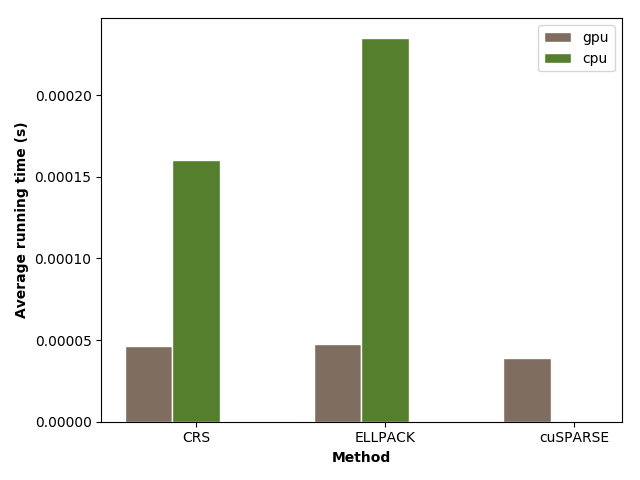
\includegraphics[width=0.8\linewidth]{running_times.png}
\label{fig:running_times} \end{figure}


\begin{table}[] 
  \centering 
  \begin{tabular}{|l|l|l|l|l|} 
    \hline Method               & Average time & 1            & 2            & 3 \\
    \hline CPU                      & 1.600510e-04 & 7.989560e-04 & 1.593470e-04 & 1.586510e-04 \\
    \hline GPU                      & 4.646400e-05 & 5.334400e-05 & 4.668800e-05 & 4.742400e-05 \\
    \hline GPU texture memory     & 4.848800e-05 & 1.091520e-04 & 5.129600e-05 & 4.912000e-05 \\
    \hline CPU managed before GPU & 1.610724e-04 & 2.447670e-04 & 2.344980e-04 & 1.753500e-04 \\
    \hline GPU managed            & 4.674400e-05 & 4.469568e-03 & 4.918400e-05 & 4.796800e-05 \\
    \hline CPU managed after GPU  & 1.610724e-04 & 2.447670e-04 & 2.344980e-04 & 1.753500e-04 \\
    \hline cuSPARSE                 & 3.886400e-05 & 1.065280e-04 & 4.323200e-05 & 3.977600e-05 \\ \hline
  \end{tabular} 
  \caption{The recorded timings for each method utilizing the CRS
    data format. The average is the average over the 10 runs excluding the first
    two runs. Only the first 3 runs are shown to highlight transfer times
  associated with managed memory.} 
\end{table}

\begin{table}[] 
  \centering 
  \begin{tabular}{|l|l|l|l|l|} 
    \hline Method                 & Average time & 1            & 2            & 3 \\
    \hline CPU                    & 2.352189e-04 & 7.101640e-04 & 3.498100e-04 & 2.545160e-04 \\
    \hline GPU                    & 4.766800e-05 & 5.331200e-05 & 4.723200e-05 & 4.729600e-05 \\
    \hline GPU texture memory     & 4.765600e-05 & 4.881280e-04 & 4.928000e-05 & 4.761600e-05 \\
    \hline CPU managed before GPU & 2.949605e-04 & 1.024591e-03 & 8.099850e-04 & 3.533850e-04 \\
    \hline GPU managed            & 4.756000e-05 & 8.975392e-03 & 5.948800e-05 & 4.678400e-05 \\
    \hline CPU managed after GPU  & 2.949605e-04 & 1.024591e-03 & 8.099850e-04 & 3.533850e-04 \\ \hline
  \end{tabular}

  \caption{The recorded timings for each method utilizing the ELLPACK data
    format.  The average is the average over the 10 runs excluding the first two
    runs.  Only the first 3 runs are shown to highlight transfer times associated
  with managed memory.} 
\end{table}

\begin{table}[] 
  \centering 
  \begin{tabular}{|l|l|} 
    \hline Method                 & Average kernel time \\
    \hline ELLPACK                & 865.07us \\
    \hline CRS                    & 260.40us \\
    \hline ELLPACK texture memory & 82.038us \\
    \hline CRS texture memory     & 43.023us \\
    \hline cuSPARSE               & 38.012us \\ \hline
  \end{tabular}
  \caption{The average running time of each
    kernel as reported by nvprof. I think these
  timings are likely wrong.}
\end{table}

\begin{table}[] 
  \centering 
  \begin{tabular}{|l|l|} 
    \hline API call           & Time \\
    \hline cudaFree           & 437.68ms \\
    \hline cudaMalloc         & 296.62ms \\
    \hline cudaMemcpy         & 30.429ms \\
    \hline cudaMallocManaged  & 20.848ms \\
    \hline cudaEventSynchroni & 16.806ms \\
    \hline cudaDeviceSynchron & 8.6555ms \\
    \hline cuDeviceGetAttribu & 1.2526ms \\
    \hline cudaLaunchKernel   & 607.89us \\
    \hline cuDeviceTotalMem   & 551.48us \\
    \hline cudaEventRecord    & 321.05us \\ \hline
  \end{tabular} 
  \caption{The total time for all API calls
  which took longer than 200 us.}
\end{table}

\end{document}
